Il sistema in analisi è stato modellato come una rete di code aperta il cui schema è riportato in \autoref{fig:queue_network_model}.\\
I job rappresentano gli utenti della WebApp dal momento in cui effettuano il login fino all'uscita successiva al checkout a seguito del pagamento.\\
Il percorso del job all'interno del sistema consiste in tre visite al centro A ed una visita ai centri B e P seguendo l'ordine: A-B-A-P-A. Dopo il terzo passaggio in A il job esce dal sistema. Per questo motivo è stata assegnata ai job una classe seguendo il seguente criterio:
\begin{itemize}
    \item \textbf{Classe 1}: sono i job che arrivano dall'esterno e restano in tale classe fino all'entrata in servizio in B.
    \item \textbf{Classe 2}: sono i job in arrivo nel server A tramite il feedback del server B e restano in tale classe fino all'entrata in servizio in P
    \item \textbf{Classe 3}: sono i job in arrivo nel server A tramite il feedback del server P. Sono anche la classe di job che escono dal sistema.
\end{itemize}
Con questa premessa le variabili di stato che meglio descrivono il sistema sono di due tipologie:
\begin{itemize}
    \item $N_{node,\ class}$: numero di job di classe $class \in \{1,2,3\}$ nel nodo $node \in \{A,B,P\}$
    \item $C_j\ con\ j \in [0, \infty)$: valore che indica la classe di appartenenza del job j.
\end{itemize}
La simulazione utilizzata è una \textit{next-event simulation}. Gli eventi sono di due tipologie, arrivi (Arrival) caratterizzati da server di destinazione e classe del job in arrivo e partenze (Departure) caratterizzato da server di partenza e classe del job in partenza. Non abbiamo inserito nessun evento artificiale\\
Di seguito l'evoluzione del sistema in base al verificarsi degli eventi divisi per server.\\
\textbf{Server A}
\begin{itemize}
    \item Arrivo dall'esterno del sistema: vengono modificate le variabile di stato incrementando $N_A,1$ e ponendo $C_j=1$. Vengono generati l'evento di Departure per il job di classe 1 dal server A e l'evento di arrival dall'esterno successivo;
    \item Departure di job di calsse 1: viene decrementata la variabile di stato $N_A,1$ e generato l'arrivo del job di classe 1 nel server B;
    \item Arrival di job di classe 2: viene incrementata la variabile di stato $N_A,2$, viene generato l'evento di Departure per il job di classe 2 dal server A.
    \item Departure di job di classe 2: viene decrementata la variabile di stato $N_A,2$. Viene generato l'arrivo del job di classe 2 nel server P;
    \item Arrival di job di classe 3: viene incrementata la variabile di stato $N_A,3$, viene generato l'evento di Departure per il job di classe 3 dal server A.
    \item Departure di job di classe 3: E' l'evento di uscita dal sistema. Viene decrementata la variabile di stato $N_A,3$.
\end{itemize}
\textbf{Server B}
\begin{itemize}
    \item Arrival di job di classe 1: viene incrementata la variabile di stato $N_B,1$, viene generato l'evento di Departure per il job di classe 1 dal server B.
    \item Departure di job di classe 1: vengono modificate le variabile di stato decrementando $N_B,1$ e ponendo $C_j=2$. Viene generato l'arrivo del job di classe 2 nel server A;
\end{itemize}
\textbf{Server P}
\begin{itemize}
    \item Arrival di job di classe 2: viene incrementata la variabile di stato $N_P,2$, viene generato l'evento di Departure per il job di classe 2 dal server P.
    \item Departure di job di classe 2: vengono modificate le variabile di stato decrementando $N_P,2$ e ponendo $C_j=3$. Viene generato l'arrivo del job di classe 3 nel server P;
\end{itemize}

\begin{figure}
    \centering
    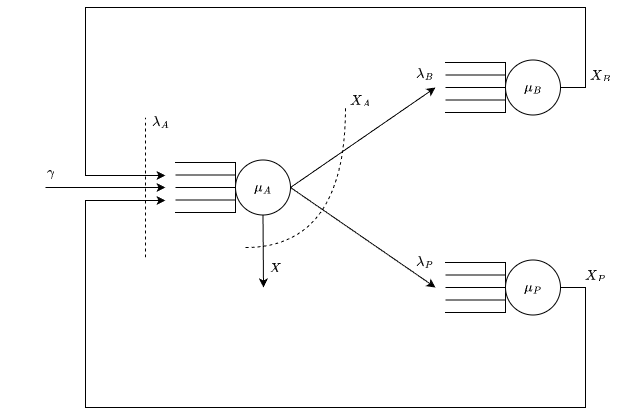
\includegraphics[width=\linewidth]{figs/webapp_conceptual.drawio.png}
    \caption{Diagramma del modello a reti di code del sistema}
    \label{fig:queue_network_model}
\end{figure}